\subsection{Autenticação Básica HTTP}

A Autenticação Básica HTTP (\emph{Hypertext Transfer Protocol}) foi definida na especificação
HTTP/1.0 \cite{RFC1945}, porém foi realocada para a RFC 2617 \cite{RFC2617}. Neste tipo de
autenticação, o servidor web recusa uma transação caso o cliente não esteja autenticado,
desafiando-o para obter um nome de usuário e senha válidos. Este desafio de autenticação é iniciado
retornando o status HTTP 401 (não autorizado) e especificando o domínio de segurança
(\emph{security realm}) a ser acessado, com o cabeçalho \texttt{WWW-Authenticate}. Ao receber o 
desafio, o cliente abre uma caixa de diálogo para que o usuário insira as credenciais para acesso 
ao domínio. O cliente então junta as informações de usuário e senha, colocando dois pontos entre 
eles, e os codifica usando o método de codificação base-64. Estas credenciais codificadas são 
colocadas no cabeçalho \texttt{Authorization}, e então a requisição é enviada para o servidor, que 
fará a validação das credenciais e, caso validadas, retorna-se o status HTTP 200 (OK) 
\cite{GOURLEY2002}. Um exemplo do funcionamento deste método de autenticação é mostrado na Figura 
\ref{fig:basicAuth}.

\begin{figure}[ht]
  \centering
  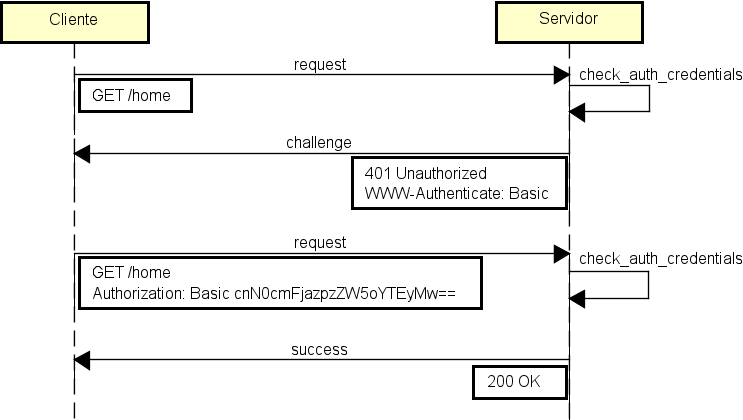
\includegraphics[width=.8\textwidth]{Basic Authentication.png}
  \caption{Exemplo de Autenticação Básica HTTP}
  \label{fig:basicAuth}
\end{figure}

A diretiva de domínio (\emph{realm}) utilizada nas autenticações HTTP define os espaços de proteção 
do sistema web. Esses domínios permitem que os recursos protegidos sejam particionados, cada um com 
seu próprio esquema de autenticação e/ou autorização \cite{RFC2617}.

A Autenticação Básica HTTP é simples e de fácil implementação, porém não possui segurança. As 
credenciais do usuário podem ser facilmente decodificadas, visto que a codificação base64 é 
facilmente reversível, podendo ser realizada em poucos segundos. Também é possível realizar ataques 
de reprodução, visto que terceiros podem capturar pacotes e replicá-los, mesmo que codificados, 
podendo obter acesso ao sistema. Este tipo de autenticação não possui proteção contra \emph{proxies} 
ou \emph{middlewares}, que podem facilmente modificar o corpo da mensagem, e também são vulneráveis 
a servidores falsificados, que se passam por outros para realizar o roubo de credenciais 
\cite{GOURLEY2002}. Além destes pontos negativos a autenticação básica é \emph{stateless} (sem estado), cada solicitação é tratada separadamente, sem conexão contínua entre elas. Isso faz com que, enquanto possuir os dados, o cliente continuará mandando os cabeçalhos de autenticação em todas as requisições HTTP subsequentes para o mesmo domínio.